\documentclass[tikz]{standalone}

\usepackage{mathtools}

\let\Im\relax
\DeclareMathOperator{\Im}{Im}
\let\Re\relax
\DeclareMathOperator{\Re}{Re}

\usetikzlibrary{decorations.markings,positioning}

\providecommand{\poles}{
  \node (poles) at (2.75,1.5) {poles of $h(p_0)$};
  \draw[fill]
  (1.5,3) coordinate [circle,fill,inner sep=1pt,label=right:$p_1$] (p1)
  (2,-2) coordinate [circle,fill,inner sep=1pt,label=below:$p_2$] (p2)
  (-3,1) coordinate [circle,fill,inner sep=1pt,label=above:$p_3$] (p3)
  (-2,-1.5) coordinate [circle,fill,inner sep=1pt,label=above:$p_4$] (p4);
  \draw[ultra thin,gray] (poles) -- (p1) (poles) -- (p2) (poles.west) -- (p3) (poles) -- (p4);
}

\def\xr{3}
\def\yr{3}

\begin{document}
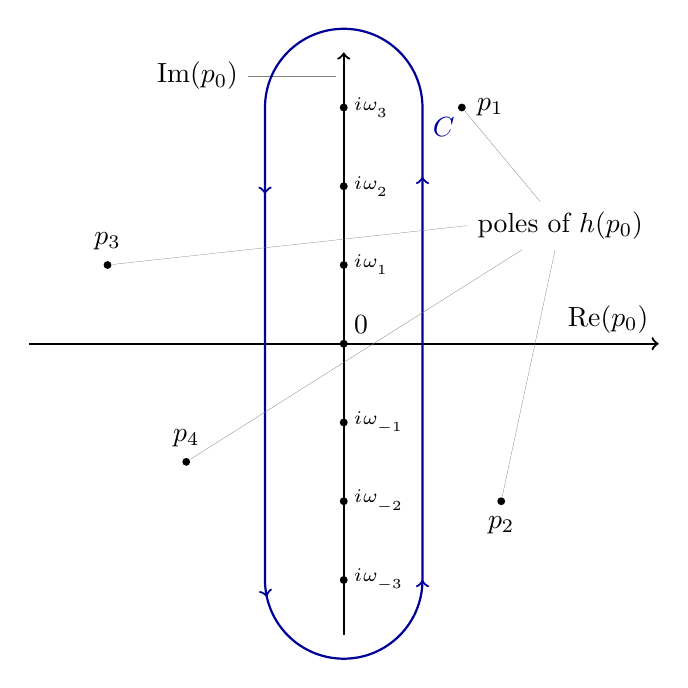
\begin{tikzpicture}[thick]

  % Axes
  \draw [->] (-\xr-1,0) -- (\xr+1,0) node [above left] {$\Re(p_0)$};
  \draw [->] (0,-\yr-0.7) -- (0,\yr+0.7) coordinate [below left = 0.3 and 0.1] (y-axis);
  \node (y-label) at ([xshift=-50]y-axis) {$\Im(p_0)$};
  \draw[ultra thin,gray] (y-axis) -- (y-label);

  % Matsubara frequencies
  \foreach \n in {-\yr,...,-1,1,2,...,\yr}{%
      \draw[fill] (0,\n) circle (1pt) node [right,font=\scriptsize] {$i \mkern1mu \omega_{_{\n}}$};}
  \draw[fill] (0,0) circle (1pt) node [above right] {0};

  % Contour line
  \draw[blue!60!black,decoration={markings,mark=between positions 0 and 1 step 0.28 with \arrow{>}},postaction={decorate}] (1,-\yr) -- (1,\yr) node [below right] {$C$} arc (0:180:1) (-1,\yr) -- (-1,-\yr) arc (180:360:1);

  % Poles of h(p_0)
  \poles

\end{tikzpicture}
\end{document}
